% Options for packages loaded elsewhere
\PassOptionsToPackage{unicode}{hyperref}
\PassOptionsToPackage{hyphens}{url}
\PassOptionsToPackage{dvipsnames,svgnames,x11names}{xcolor}
%
\documentclass[
  10pt,
]{article}
\usepackage{amsmath,amssymb}
\usepackage{iftex}
\ifPDFTeX
  \usepackage[T1]{fontenc}
  \usepackage[utf8]{inputenc}
  \usepackage{textcomp} % provide euro and other symbols
\else % if luatex or xetex
  \usepackage{unicode-math} % this also loads fontspec
  \defaultfontfeatures{Scale=MatchLowercase}
  \defaultfontfeatures[\rmfamily]{Ligatures=TeX,Scale=1}
\fi
\usepackage{lmodern}
\ifPDFTeX\else
  % xetex/luatex font selection
\fi
% Use upquote if available, for straight quotes in verbatim environments
\IfFileExists{upquote.sty}{\usepackage{upquote}}{}
\IfFileExists{microtype.sty}{% use microtype if available
  \usepackage[]{microtype}
  \UseMicrotypeSet[protrusion]{basicmath} % disable protrusion for tt fonts
}{}
\makeatletter
\@ifundefined{KOMAClassName}{% if non-KOMA class
  \IfFileExists{parskip.sty}{%
    \usepackage{parskip}
  }{% else
    \setlength{\parindent}{0pt}
    \setlength{\parskip}{6pt plus 2pt minus 1pt}}
}{% if KOMA class
  \KOMAoptions{parskip=half}}
\makeatother
\usepackage{xcolor}
\usepackage[margin=0.8in]{geometry}
\usepackage{color}
\usepackage{fancyvrb}
\newcommand{\VerbBar}{|}
\newcommand{\VERB}{\Verb[commandchars=\\\{\}]}
\DefineVerbatimEnvironment{Highlighting}{Verbatim}{commandchars=\\\{\}}
% Add ',fontsize=\small' for more characters per line
\newenvironment{Shaded}{}{}
\newcommand{\AlertTok}[1]{\textcolor[rgb]{1.00,0.00,0.00}{\textbf{#1}}}
\newcommand{\AnnotationTok}[1]{\textcolor[rgb]{0.38,0.63,0.69}{\textbf{\textit{#1}}}}
\newcommand{\AttributeTok}[1]{\textcolor[rgb]{0.49,0.56,0.16}{#1}}
\newcommand{\BaseNTok}[1]{\textcolor[rgb]{0.25,0.63,0.44}{#1}}
\newcommand{\BuiltInTok}[1]{\textcolor[rgb]{0.00,0.50,0.00}{#1}}
\newcommand{\CharTok}[1]{\textcolor[rgb]{0.25,0.44,0.63}{#1}}
\newcommand{\CommentTok}[1]{\textcolor[rgb]{0.38,0.63,0.69}{\textit{#1}}}
\newcommand{\CommentVarTok}[1]{\textcolor[rgb]{0.38,0.63,0.69}{\textbf{\textit{#1}}}}
\newcommand{\ConstantTok}[1]{\textcolor[rgb]{0.53,0.00,0.00}{#1}}
\newcommand{\ControlFlowTok}[1]{\textcolor[rgb]{0.00,0.44,0.13}{\textbf{#1}}}
\newcommand{\DataTypeTok}[1]{\textcolor[rgb]{0.56,0.13,0.00}{#1}}
\newcommand{\DecValTok}[1]{\textcolor[rgb]{0.25,0.63,0.44}{#1}}
\newcommand{\DocumentationTok}[1]{\textcolor[rgb]{0.73,0.13,0.13}{\textit{#1}}}
\newcommand{\ErrorTok}[1]{\textcolor[rgb]{1.00,0.00,0.00}{\textbf{#1}}}
\newcommand{\ExtensionTok}[1]{#1}
\newcommand{\FloatTok}[1]{\textcolor[rgb]{0.25,0.63,0.44}{#1}}
\newcommand{\FunctionTok}[1]{\textcolor[rgb]{0.02,0.16,0.49}{#1}}
\newcommand{\ImportTok}[1]{\textcolor[rgb]{0.00,0.50,0.00}{\textbf{#1}}}
\newcommand{\InformationTok}[1]{\textcolor[rgb]{0.38,0.63,0.69}{\textbf{\textit{#1}}}}
\newcommand{\KeywordTok}[1]{\textcolor[rgb]{0.00,0.44,0.13}{\textbf{#1}}}
\newcommand{\NormalTok}[1]{#1}
\newcommand{\OperatorTok}[1]{\textcolor[rgb]{0.40,0.40,0.40}{#1}}
\newcommand{\OtherTok}[1]{\textcolor[rgb]{0.00,0.44,0.13}{#1}}
\newcommand{\PreprocessorTok}[1]{\textcolor[rgb]{0.74,0.48,0.00}{#1}}
\newcommand{\RegionMarkerTok}[1]{#1}
\newcommand{\SpecialCharTok}[1]{\textcolor[rgb]{0.25,0.44,0.63}{#1}}
\newcommand{\SpecialStringTok}[1]{\textcolor[rgb]{0.73,0.40,0.53}{#1}}
\newcommand{\StringTok}[1]{\textcolor[rgb]{0.25,0.44,0.63}{#1}}
\newcommand{\VariableTok}[1]{\textcolor[rgb]{0.10,0.09,0.49}{#1}}
\newcommand{\VerbatimStringTok}[1]{\textcolor[rgb]{0.25,0.44,0.63}{#1}}
\newcommand{\WarningTok}[1]{\textcolor[rgb]{0.38,0.63,0.69}{\textbf{\textit{#1}}}}
\usepackage{longtable,booktabs,array}
\usepackage{calc} % for calculating minipage widths
% Correct order of tables after \paragraph or \subparagraph
\usepackage{etoolbox}
\makeatletter
\patchcmd\longtable{\par}{\if@noskipsec\mbox{}\fi\par}{}{}
\makeatother
% Allow footnotes in longtable head/foot
\IfFileExists{footnotehyper.sty}{\usepackage{footnotehyper}}{\usepackage{footnote}}
\makesavenoteenv{longtable}
\usepackage{graphicx}
\makeatletter
\def\maxwidth{\ifdim\Gin@nat@width>\linewidth\linewidth\else\Gin@nat@width\fi}
\def\maxheight{\ifdim\Gin@nat@height>\textheight\textheight\else\Gin@nat@height\fi}
\makeatother
% Scale images if necessary, so that they will not overflow the page
% margins by default, and it is still possible to overwrite the defaults
% using explicit options in \includegraphics[width, height, ...]{}
\setkeys{Gin}{width=\maxwidth,height=\maxheight,keepaspectratio}
% Set default figure placement to htbp
\makeatletter
\def\fps@figure{htbp}
\makeatother
\setlength{\emergencystretch}{3em} % prevent overfull lines
\providecommand{\tightlist}{%
  \setlength{\itemsep}{0pt}\setlength{\parskip}{0pt}}
\setcounter{secnumdepth}{5}
\ifLuaTeX
  \usepackage{selnolig}  % disable illegal ligatures
\fi
\IfFileExists{bookmark.sty}{\usepackage{bookmark}}{\usepackage{hyperref}}
\IfFileExists{xurl.sty}{\usepackage{xurl}}{} % add URL line breaks if available
\urlstyle{same}
\hypersetup{
  pdftitle={LuSIR: Latent Upscaling via Self-trained Image Restoration without T2I Pretraining},
  colorlinks=true,
  linkcolor={blue},
  filecolor={Maroon},
  citecolor={Blue},
  urlcolor={blue},
  pdfcreator={LaTeX via pandoc}}

\title{LuSIR: Latent Upscaling via Self-trained Image Restoration
without T2I Pretraining}
\author{}
\date{}

\begin{document}
\maketitle

{
\hypersetup{linkcolor=}
\setcounter{tocdepth}{3}
\tableofcontents
}
Snapshot: masked detail branch v2 and its formal x4 benchmark are
complete, Stage 2 clean-fidelity learning-rate probes are complete, the
Stage 2 detail-perceptual continuation has been formally reviewed but
not promoted, and several deterministic/generative visible-detail probes
were evaluated without producing a clear texture breakthrough.

\texttt{paper/TECHNICAL\_REPORT.md} is the canonical report source.
\texttt{paper/sr\_diffusion\_report.pdf} and \texttt{paper/main.tex} are
generated from it with \texttt{paper/build\_report.sh}, so the Markdown
and PDF contain the same report.

\hypertarget{objective}{%
\section{Objective}\label{objective}}

LuSIR trains a vision-only x4 latent diffusion super-resolution model
without using a pretrained text-to-image backbone. The active task is:

\begin{Shaded}
\begin{Highlighting}[]
\NormalTok{LR 128x128 {-}\textgreater{} HR 512x512}
\end{Highlighting}
\end{Shaded}

The model path is:

\begin{Shaded}
\begin{Highlighting}[]
\NormalTok{HR image {-}\textgreater{} factor{-}4 VAE {-}\textgreater{} HR latent}
\NormalTok{LR image {-}\textgreater{} condition encoder {-}\textgreater{} condition latent}
\NormalTok{noisy HR latent + condition latent + timestep + domain id {-}\textgreater{} conditional U{-}Net}
\NormalTok{denoised latent {-}\textgreater{} VAE decoder {-}\textgreater{} SR output}
\end{Highlighting}
\end{Shaded}

The numbered stages describe training order, not a mandatory Stage 1
-\textgreater{} 2 -\textgreater{} 3 -\textgreater{} 4 runtime chain. The
current runtime choices are:

\begin{Shaded}
\begin{Highlighting}[]
\NormalTok{public Colab default:}
\NormalTok{  LR {-}\textgreater{} Stage 2 XL condition encoder {-}\textgreater{} residual refiner v2 {-}\textgreater{} Stage 1 decoder}

\NormalTok{current detail research candidate:}
\NormalTok{  LR {-}\textgreater{} dual{-}context LSDIR Stage 2 {-}\textgreater{} Stage 1 decoder}
\NormalTok{     {-}\textgreater{} learned detail mask {-}\textgreater{} masked detail branch v2}

\NormalTok{generative comparison:}
\NormalTok{  LR {-}\textgreater{} Stage 2 condition encoder {-}\textgreater{} Stage 3 OR Stage 4 diffusion U{-}Net}
\NormalTok{     {-}\textgreater{} Stage 1 decoder}
\end{Highlighting}
\end{Shaded}

Stage 4 is a Stage 3-derived replacement diffusion checkpoint. It does
not run after Stage 3. Planned Stage 5 distillation would similarly
replace the slower diffusion sampler rather than append another serial
module.

\hypertarget{data}{%
\section{Data}\label{data}}

The base photo100k split has 103,450 training images and 100 fixed
validation images. The completed dual-context Stage 2 scale-up adds
30,000 unique LSDIR training images, for 133,450 unique training images
and the unchanged 100-image validation set. LR inputs are generated on
the fly from HR crops. Earlier XL work used
\texttt{photo\_v3\_noise\_mix}, a strong denoise-focused curriculum with
no clean share and 80\% combined v2/v3 cases. Later work introduced
\texttt{photo\_detail\_mix}: 35\% clean, 48\% detail-preserving photo
degradation, 15\% mild degradation, and 2\% strong \texttt{photo\_v2}.
This keeps a small robustness tail while shifting the primary objective
toward user-facing detail restoration.

\hypertarget{completed-baselines}{%
\section{Completed Baselines}\label{completed-baselines}}

\begin{longtable}[]{@{}lll@{}}
\toprule\noalign{}
Stage & Run & Result \\
\midrule\noalign{}
\endhead
\bottomrule\noalign{}
\endlastfoot
Stage 1 VAE & \texttt{autoencoder\_photo10k\_b16\_eval\_online} &
\texttt{eval/psnr\ 40.19} \\
Stage 2 photo100k & \texttt{latent\_pretrain\_photo100k\_b64} & best
latent loss \texttt{0.21230} \\
Stage 3 photo100k & \texttt{diffusion\_photo100k\_b32} & sampled val100
\texttt{25.3745} PSNR \\
Stage 4 photo100k &
\texttt{diffusion\_photo100k\_b32\_stage4\_condition} & sampled val100
\texttt{25.4072} PSNR \\
Stage 4 photo100k v2 &
\texttt{diffusion\_photo100k\_b32\_stage4\_condition\_v2} & sampled
val100 \texttt{22.8426} PSNR, \texttt{+0.4323} over bicubic \\
\end{longtable}

The v2 task has a stronger degradation distribution, so its absolute
PSNR is not directly comparable with the earlier mild photo100k run.

\hypertarget{exploratory-strict-bicubic-five-image-comparison}{%
\section{Exploratory Strict-Bicubic Five-Image
Comparison}\label{exploratory-strict-bicubic-five-image-comparison}}

The ordinary LuSIR validation metrics use task-specific degradations, so
their absolute PSNR values should not be compared directly with
published bicubic-only SR benchmarks. A small strict-bicubic diagnostic
was added to separate degradation difficulty from reconstruction
capacity. The new \texttt{benchmark\_bicubic} preset applies only PIL
bicubic factor-4 downsampling and does not add blur, noise, compression,
color changes, or sharpening.

The shared diagnostic protocol is:

\begin{Shaded}
\begin{Highlighting}[]
\NormalTok{source images: DIV2K validation 0801{-}0805}
\NormalTok{HR input: deterministic center 512x512 crop}
\NormalTok{LR input: strict PIL bicubic x4 downsample to 128x128}
\NormalTok{metric: mean per{-}image RGB PSNR over the full 512x512 crop}
\NormalTok{deterministic inference: CPU FP32}
\NormalTok{diffusion inference: condition initialization, start timestep 50, 32 DDIM steps}
\end{Highlighting}
\end{Shaded}

Loaded parameter counts include the entire 21.10M-parameter Stage 1 VAE
because the current runners load the full module, although inference
executes only its 10.52M-parameter decoder. This matches the existing
\texttt{509.658M} Stage 4 XL accounting.

\begin{longtable}[]{@{}lrrrr@{}}
\toprule\noalign{}
Inference path & Selected checkpoint & Loaded params & Mean RGB PSNR &
vs bicubic \\
\midrule\noalign{}
\endhead
\bottomrule\noalign{}
\endlastfoot
Bicubic & n/a & n/a & \texttt{29.5999} & n/a \\
Stage 2 XL condition-only & step 72000 & \texttt{40.040M} &
\texttt{30.5677} & \texttt{+0.9678} \\
Stage 2 XL + residual refiner v2 & step 39000 & \texttt{48.106M} &
\texttt{30.8205} & \texttt{+1.2206} \\
Stage 2 multiscale & step 46000 & \texttt{76.591M} & \texttt{31.6068} &
\texttt{+2.0069} \\
Stage 2 dual-context LSDIR & step 98000 & \texttt{140.334M} &
\texttt{31.7411} & \texttt{+2.1412} \\
Dual-context + detail v1b & step 39500 & \texttt{141.675M} &
\texttt{31.8135} & \texttt{+2.2136} \\
Dual-context + detail v1c & step 6000 & \texttt{141.689M} &
\texttt{31.8154} & \texttt{+2.2155} \\
Dual-context + detail v1d & step 99500 & \texttt{143.354M} &
\texttt{31.9513} & \texttt{+2.3514} \\
Stage 4 XL edge, 32-step sampled & step 4250 & \texttt{509.658M} &
\texttt{29.5487} & \texttt{-0.0512} \\
\end{longtable}

The strict-bicubic result confirms that LuSIR already operates in the
30-32 dB range when the LR input is not additionally corrupted. The much
lower \texttt{photo\_detail\_mix} and strong-preset values primarily
reflect degradation difficulty rather than a direct 6-7 dB gap to
bicubic-only SR papers.

The capacity trend is also informative. Stage 2 XL to multiscale gains
\texttt{+1.0391\ dB}, and multiscale to dual-context gains another
\texttt{+0.1343\ dB}. The detail branches then provide smaller but
consistent gains over dual-context: v1b \texttt{+0.0725\ dB}, v1c
\texttt{+0.0744\ dB}, and the completed 3.02M v1d \texttt{+0.2102\ dB}.
V1d improves v1c by \texttt{+0.1358\ dB} after three epochs. This
confirms that the long capacity run was useful, but the visual change
remains conservative and is not a perceptual-detail breakthrough.

The 509.7M Stage 4 XL edge checkpoint is the clearest counterexample to
treating parameter count as a quality ranking. On this clean bicubic
diagnostic it falls \texttt{-0.0512\ dB} below bicubic and
\texttt{-1.0190\ dB} below its own Stage 2 XL condition-only path.
Visual inspection shows that it can add apparent sharpness, but it also
changes clean input details enough to reduce reconstruction fidelity.
This is consistent with its strong-noise denoise/color-cleanup training
role; it should not be routed unconditionally for clean inputs.

This diagnostic is deliberately small and is not a published-benchmark
claim. It uses five center crops, RGB PSNR, no border shave, and PIL
bicubic rather than the full-image Y-channel/Matlab-bicubic conventions
used by many SR papers. The formal full-image benchmark described next
supersedes it for clean-bicubic fidelity comparison.

The machine-readable snapshot is stored in:

\begin{Shaded}
\begin{Highlighting}[]
\NormalTok{metrics/benchmark\_bicubic5\_lusir\_model\_comparison.json}
\end{Highlighting}
\end{Shaded}

\hypertarget{formal-full-image-x4-benchmark}{%
\section{Formal Full-Image x4
Benchmark}\label{formal-full-image-x4-benchmark}}

A formal evaluator now measures full-image DIV2K validation, Set5,
Set14, and Urban100 using their public x4 bicubic LR pairs. It uses
MATLAB-compatible BT.601 Y conversion, a four-pixel border shave, and
MATLAB-style SSIM. All candidate outputs are required to match the HR
dimensions exactly; the evaluator never hides an error by resizing an
output.

\begin{longtable}[]{@{}lrrrr@{}}
\toprule\noalign{}
Candidate & DIV2K & Set5 & Set14 & Urban100 \\
\midrule\noalign{}
\endhead
\bottomrule\noalign{}
\endlastfoot
Bicubic & 28.1044 & 28.4318 & 26.0928 & 23.1412 \\
RealESRNet x4plus & 28.8250 & 29.3828 & 27.1465 & 24.4613 \\
RealESRGAN x4plus & 26.6125 & 26.6160 & 25.4216 & 22.6709 \\
SwinIR classical x4 & \textbf{31.0838} & not run & not run & not run \\
LuSIR refiner v2 & 28.7857 & 28.1896 & 27.3704 & 24.9176 \\
LuSIR dual-context base & 29.9575 & 31.6621 & 28.2441 & 25.4816 \\
\textbf{LuSIR detail v1d} & \textbf{30.1602} & \textbf{31.8892} &
\textbf{28.4123} & \textbf{25.8755} \\
\textbf{LuSIR masked detail v2} & \textbf{30.1636} & \textbf{31.9495} &
\textbf{28.4257} & \textbf{25.8922} \\
\end{longtable}

The table reports Y PSNR; full Y SSIM and RGB PSNR values are preserved
in the machine-readable results. V1d improves the frozen dual-context
base on all four datasets. Its Y PSNR gains are \texttt{+0.2027},
\texttt{+0.2271}, \texttt{+0.1682}, and \texttt{+0.3939\ dB},
respectively. Its Y SSIM is \texttt{0.83421}, \texttt{0.89440},
\texttt{0.77998}, and \texttt{0.77875}. This validates the branch
redesign under a standard full-image protocol, with the strongest gain
on texture-heavy Urban100.

The official SwinIR classical x4 checkpoint reaches
\texttt{31.0838\ /\ 0.85228} on the same DIV2K evaluator. It is
\texttt{+0.9235\ dB} Y PSNR and \texttt{+0.01807} Y SSIM ahead of detail
v1d. The detail branch is doing useful corrective work, but this
remaining gap identifies the Stage 2/base reconstruction path as the
primary clean-fidelity bottleneck.

RealESRNet and RealESRGAN target real-world degradation and perceptual
quality, so their clean-bicubic fidelity scores do not establish a
general visual quality ranking. Likewise, beating these checkpoints
under this protocol does not establish classical-SR SOTA. A classical
fidelity baseline, perceptual metrics, real-degradation evaluation, and
blind human review remain necessary. The reproducible protocol and
commands are in \texttt{docs/SR\_BENCHMARK.md}; full machine-readable
results are in:

\begin{Shaded}
\begin{Highlighting}[]
\NormalTok{metrics/formal\_x4\_benchmark\_lusir\_realesr\_summary.json}
\NormalTok{metrics/formal\_x4\_benchmark\_lusir\_realesr\_metrics.csv}
\NormalTok{metrics/formal\_x4\_benchmark\_div2k\_swinir\_summary.json}
\NormalTok{metrics/formal\_x4\_benchmark\_div2k\_swinir\_metrics.csv}
\NormalTok{metrics/formal\_x4\_benchmark\_detail\_v2\_masked\_summary.json}
\NormalTok{metrics/formal\_x4\_benchmark\_detail\_v2\_masked\_metrics.csv}
\NormalTok{metrics/formal\_x4\_benchmark\_stage2\_detail\_perceptual\_v1\_summary.json}
\NormalTok{metrics/formal\_x4\_benchmark\_stage2\_detail\_perceptual\_v1\_metrics.csv}
\end{Highlighting}
\end{Shaded}

\hypertarget{stage-2-clean-fidelity-continuation-and-learning-rate-probes}{%
\section{Stage 2 Clean-Fidelity Continuation and Learning-Rate
Probes}\label{stage-2-clean-fidelity-continuation-and-learning-rate-probes}}

The clean-bicubic continuation starts from dual-context Stage 2
best98000 and uses \texttt{benchmark\_bicubic} with a PSNR-oriented
decoded loss balance. Its task-specific val100 decoded-PSNR proxy
improved gradually:

\begin{longtable}[]{@{}rr@{}}
\toprule\noalign{}
Step & Decoded PSNR proxy \\
\midrule\noalign{}
\endhead
\bottomrule\noalign{}
\endlastfoot
1000 & \texttt{25.019} \\
4000 & \texttt{25.031} \\
9000 & \texttt{25.045} \\
15000 & \textbf{\texttt{25.057}} \\
17000 & \texttt{25.054} \\
\end{longtable}

The run was stopped manually at step 17825 after no new best beyond step
15000. Its checkpoints remain available for future clean-fidelity work.

These values are not directly comparable with the formal full-image
Y-channel results. The formal DIV2K comparison is LuSIR masked detail v2
at \texttt{30.1636\ dB} and SwinIR classical x4 at \texttt{31.0838\ dB}.

Separate learning-rate probes preserved the original step-15000
checkpoint. A \texttt{20x} continuation collapsed to \texttt{15.72\ dB}
at its first evaluation. A \texttt{5x} continuation remained below the
original run, while a \texttt{5x} from-initialization run reached
\texttt{25.033\ dB} at step 4000 versus \texttt{25.031\ dB} for the
original learning rate. The difference is too small to treat as a gain.
The original \texttt{5e-6} learning rate is retained, and learning-rate
scarcity is rejected as the main bottleneck.

The result also clarifies the objective boundary. Same-objective Stage 2
continuation can refine deterministic fidelity, but it is unlikely to
produce the visibly new fine texture expected from a generative model.

\hypertarget{stage-2-detail-perceptual-continuation-review}{%
\section{Stage 2 Detail-Perceptual Continuation
Review}\label{stage-2-detail-perceptual-continuation-review}}

A separate Stage 2 continuation started from dual-context best98000 and
trained on \texttt{photo\_detail\_mix} with lower latent/decoded weight,
stronger highpass magnitude, VGG feature loss, and a detail-score
selection metric:

\begin{Shaded}
\begin{Highlighting}[]
\NormalTok{config: configs/latent\_pretrain\_photo130k\_lsdir\_dual\_detail\_perceptual\_v1.yaml}
\NormalTok{run:    /home/ubuntu/scratch/sr{-}diffusion/runs/latent\_pretrain\_photo130k\_lsdir\_dual\_detail\_perceptual\_v1}
\NormalTok{W\&B:    https://wandb.ai/jwheo/LuSIR/runs/hybqq4rj}
\end{Highlighting}
\end{Shaded}

The val100 proxy confirmed that the loss can raise high-frequency
energy: step6000 reached decoded PSNR \texttt{24.5921} with Laplacian
energy ratio \texttt{0.3824}, and latest step12000 reached decoded PSNR
\texttt{24.6144} with ratio \texttt{0.3533}. The original dual-context
step98000 baseline on the same proxy was \texttt{24.6197} and
\texttt{0.3123}.

The decisive review used the same 219-image formal x4 benchmark as
above, but with the Stage 2 base path only:

\begin{longtable}[]{@{}lrrrr@{}}
\toprule\noalign{}
Candidate & Mean Y PSNR & Mean Y SSIM & Mean RGB PSNR & Mean RGB SSIM \\
\midrule\noalign{}
\endhead
\bottomrule\noalign{}
\endlastfoot
Bicubic & \texttt{25.7170} & \texttt{0.71773} & \texttt{24.2697} &
\texttt{0.69205} \\
Dual-context step98000 & \textbf{\texttt{27.8431}} & \texttt{0.79742} &
\textbf{\texttt{26.3131}} & \texttt{0.77340} \\
Detail-perceptual step6000 & \texttt{27.7737} &
\textbf{\texttt{0.79914}} & \texttt{26.2482} &
\textbf{\texttt{0.77506}} \\
Detail-perceptual latest12000 & \texttt{27.8356} & \texttt{0.79827} &
\texttt{26.3107} & \texttt{0.77417} \\
\end{longtable}

Relative to dual-context step98000, step6000 loses \texttt{0.0694\ dB} Y
PSNR while gaining \texttt{0.00172} Y SSIM. Latest step12000 is almost
tied: \texttt{-0.0076\ dB} Y PSNR, \texttt{+0.00085} Y SSIM, and
\texttt{156/219} Y-SSIM wins. Dataset-level latest12000 deltas are
\texttt{-0.0193\ dB} on DIV2K, \texttt{+0.0272\ dB} on Set5,
\texttt{-0.0555\ dB} on Set14, and \texttt{+0.0092\ dB} on Urban100.

Visual crop review shows small improvements on some building/window grid
regions, but not a clear user-visible texture breakthrough. The
conclusion is therefore conservative: keep dual-context step98000 as the
default Stage 2 checkpoint, preserve latest12000 as an optional
SSIM/detail-biased research candidate, and avoid spending the next run
on a longer continuation of the same objective.

The new machine-readable results and visual crop sheet are:

\begin{Shaded}
\begin{Highlighting}[]
\NormalTok{metrics/formal\_x4\_benchmark\_stage2\_detail\_perceptual\_v1\_summary.json}
\NormalTok{metrics/formal\_x4\_benchmark\_stage2\_detail\_perceptual\_v1\_metrics.csv}
\NormalTok{metrics/formal\_x4\_benchmark\_stage2\_detail\_perceptual\_v1\_delta\_crop\_selection.csv}
\NormalTok{samples/stage2\_detail\_perceptual\_v1\_benchmark\_delta\_crop\_sheet.jpg}
\end{Highlighting}
\end{Shaded}

The first separate generative probe is
\texttt{configs/diffusion\_photo130k\_lsdir\_highfreq\_residual\_v1\_b8.yaml}.
It freezes the dual-context Stage 2 base and Stage 1 decoder, then
trains a 76.6M gated/bounded residual U-Net with strong high-frequency
supervision and a lowpass anchor. The output layer is zero-initialized:
the smoke-test prediction and condition images were byte-identical, with
zero latent residual and zero decoded drift before the first optimizer
update.

\hypertarget{stage-2-xl-candidate-selection}{%
\section{Stage 2 XL Candidate
Selection}\label{stage-2-xl-candidate-selection}}

The XL condition encoder uses:

\begin{Shaded}
\begin{Highlighting}[]
\NormalTok{config: configs/latent\_pretrain\_photo100k\_v3\_noise\_xl.yaml}
\NormalTok{base\_channels: 256}
\NormalTok{num\_blocks: 16}
\NormalTok{degradation: photo\_v3\_noise\_mix}
\NormalTok{finished step: 80000}
\end{Highlighting}
\end{Shaded}

Candidate comparison on the same validation images:

\begin{longtable}[]{@{}lrrrr@{}}
\toprule\noalign{}
Candidate & Step & Latent loss & Latent MSE & Decoded PSNR \\
\midrule\noalign{}
\endhead
\bottomrule\noalign{}
\endlastfoot
\texttt{best\_eval\_latent} & 66000 & \texttt{0.27230} &
\texttt{0.91770} & \texttt{21.3828} \\
\texttt{step\_0072000} & 72000 & \texttt{0.27940} & \texttt{0.97295} &
\texttt{21.5241} \\
\texttt{latest} & 80000 & \texttt{0.27593} & \texttt{0.89609} &
\texttt{21.5062} \\
\end{longtable}

The 72k checkpoint was selected for Stage 4 XL because it had the best
decoded condition-only PSNR on the fixed validation set.

\hypertarget{stage-4-xl-edge-loss-result}{%
\section{Stage 4 XL Edge-Loss
Result}\label{stage-4-xl-edge-loss-result}}

The first XL diffusion run used the selected Stage 2 XL condition
encoder and partial initialization from the smaller Stage 4 v2
checkpoint.

\begin{Shaded}
\begin{Highlighting}[]
\NormalTok{config: configs/diffusion\_photo100k\_xl\_stage4\_condition\_v3\_edge\_b16.yaml}
\NormalTok{run: diffusion\_photo100k\_xl\_stage4\_condition\_v3\_edge\_b16}
\NormalTok{U{-}Net path: 469.6M parameters}
\NormalTok{full inference path: 509.658M parameters}
\NormalTok{train batch size: 16}
\NormalTok{GPUs: 2x A100{-}SXM4{-}80GB through PyTorch DDP}
\NormalTok{finished step: 5000}
\NormalTok{selected checkpoint: step 4250, best eval/decoded\_mse}
\end{Highlighting}
\end{Shaded}

Training-time best proxy:

\begin{Shaded}
\begin{Highlighting}[]
\NormalTok{step 4250}
\NormalTok{eval/decoded\_psnr: 21.9872}
\NormalTok{eval/decoded\_mse: 0.025313}
\NormalTok{eval/noise\_mse: 27.66008}
\NormalTok{eval/x0\_mse: 0.86226}
\end{Highlighting}
\end{Shaded}

Sampled validation evaluation:

\begin{Shaded}
\begin{Highlighting}[]
\NormalTok{checkpoint: best\_eval\_condition\_decoded.pt}
\NormalTok{checkpoint step: 4250}
\NormalTok{split: val}
\NormalTok{limit: 100}
\NormalTok{init: condition}
\NormalTok{start\_timestep: 50}
\NormalTok{steps: 32}
\NormalTok{mean\_bicubic\_psnr: 22.3599}
\NormalTok{mean\_sr\_psnr: 23.0793}
\NormalTok{mean\_psnr\_delta: +0.7195}
\end{Highlighting}
\end{Shaded}

The latest XL Stage 4 checkpoint is therefore better than bicubic on the
current v3 validation setup and better aligned with the desired
denoise/color cleanup behavior than the Stage 2 condition-only path. It
is still not a final restoration model: outputs remain softer than GT on
fine textures.

\hypertarget{stage-4-xl-role-split-and-gated-residual-probes}{%
\section{Stage 4 XL Role-Split and Gated-Residual
Probes}\label{stage-4-xl-role-split-and-gated-residual-probes}}

Follow-up probes tested whether Stage 4 could act as a bounded detail
refiner instead of freely overwriting the deterministic Stage 2
condition latent.

The role-split mild probe added a lowpass anchor and separated
low/high-frequency decoded losses:

\begin{Shaded}
\begin{Highlighting}[]
\NormalTok{config: configs/diffusion\_photo100k\_xl\_stage4\_condition\_v3\_rolesplit\_mild\_b8\_probe.yaml}
\NormalTok{run: diffusion\_photo100k\_xl\_stage4\_condition\_v3\_rolesplit\_mild\_b8\_probe}
\NormalTok{W\&B: https://wandb.ai/jwheo/LuSIR/runs/lrb6nco9}
\NormalTok{finished step: 8000 micro{-}steps, 2000 optimizer updates}
\NormalTok{best one{-}step checkpoint: step 7500, decoded PSNR 23.2515}
\end{Highlighting}
\end{Shaded}

Sampled mild val100 showed that role-split losses reduced some
over-editing at very low start timesteps, but the diffusion path still
damaged the Stage 2 condition output on average:

\begin{longtable}[]{@{}lrrrr@{}}
\toprule\noalign{}
Model & Start timestep & Mean SR PSNR & vs condition-only & Wins vs
condition \\
\midrule\noalign{}
\endhead
\bottomrule\noalign{}
\endlastfoot
Stage 2 XL condition-only & n/a & \texttt{25.0449} & n/a & n/a \\
Stage 4 role-split & 25 & \texttt{24.5747} & \texttt{-0.4702} &
\texttt{3/100} \\
Stage 4 role-split & 10 & \texttt{24.9185} & \texttt{-0.1264} &
\texttt{3/100} \\
Stage 4 role-split & 5 & \texttt{24.9935} & \texttt{-0.0514} &
\texttt{6/100} \\
Stage 4 role-split & 1 & \texttt{25.0335} & \texttt{-0.0114} &
\texttt{10/100} \\
\end{longtable}

The next probe changed the diffusion prediction parameterization to
\texttt{gated\_residual\_x0}. Instead of predicting the full denoised
latent, the U-Net predicts a bounded residual and gate on top of the
condition latent:

\begin{Shaded}
\begin{Highlighting}[]
\NormalTok{x0\_hat = condition + residual\_scale * tanh(residual\_logits) * sigmoid(gate\_logits + gate\_bias)}
\NormalTok{residual\_scale: 1.25}
\NormalTok{gate\_bias: 0.0}
\NormalTok{out\_channels: 32}
\end{Highlighting}
\end{Shaded}

The probe was initialized from the role-split best checkpoint with
partial initialization and stopped at step 2000 after the sampled
validation result reached condition-only parity:

\begin{Shaded}
\begin{Highlighting}[]
\NormalTok{config: configs/diffusion\_photo100k\_xl\_stage4\_condition\_v3\_gated\_residual\_mild\_b8\_probe.yaml}
\NormalTok{run: diffusion\_photo100k\_xl\_stage4\_condition\_v3\_gated\_residual\_mild\_b8\_probe}
\NormalTok{W\&B: https://wandb.ai/jwheo/LuSIR/runs/edfko8e8}
\NormalTok{best one{-}step checkpoint: step 1000}
\NormalTok{final checkpoint: step 2000}
\end{Highlighting}
\end{Shaded}

Sampled mild val100:

\begin{longtable}[]{@{}lrrrrr@{}}
\toprule\noalign{}
Model & Checkpoint & Start timestep & Mean SR PSNR & vs condition-only &
Wins vs condition \\
\midrule\noalign{}
\endhead
\bottomrule\noalign{}
\endlastfoot
Stage 2 XL condition-only & n/a & n/a & \texttt{25.0449} & n/a & n/a \\
Stage 4 gated residual & 1000 & 25 & \texttt{25.0415} & \texttt{-0.0035}
& \texttt{25/100} \\
Stage 4 gated residual & 1000 & 10 & \texttt{25.0415} & \texttt{-0.0034}
& \texttt{25/100} \\
Stage 4 gated residual & 1000 & 5 & \texttt{25.0416} & \texttt{-0.0034}
& \texttt{25/100} \\
Stage 4 gated residual & 1000 & 1 & \texttt{25.0418} & \texttt{-0.0032}
& \texttt{25/100} \\
Stage 4 gated residual & 2000 & 25 & \texttt{25.0445} & \texttt{-0.0004}
& \texttt{34/100} \\
Stage 4 gated residual & 2000 & 10 & \texttt{25.0444} & \texttt{-0.0006}
& \texttt{32/100} \\
Stage 4 gated residual & 2000 & 5 & \texttt{25.0444} & \texttt{-0.0005}
& \texttt{31/100} \\
Stage 4 gated residual & 2000 & 1 & \texttt{25.0443} & \texttt{-0.0007}
& \texttt{32/100} \\
\end{longtable}

This is a partial success. The gated residual parameterization almost
eliminated the condition damage seen in previous Stage 4 probes and
increased the number of samples beating condition-only from
\texttt{10/100} at role-split t1 to \texttt{34/100} at gated-residual
step2000 t25. However, the mean result still does not beat the Stage 2
condition-only baseline. The current interpretation is that Stage 4 has
learned a safe near-identity residual path, not a reliable
missing-detail generator.

\hypertarget{stage-2-residual-diagnostic-and-deterministic-refiner}{%
\section{Stage 2 Residual Diagnostic and Deterministic
Refiner}\label{stage-2-residual-diagnostic-and-deterministic-refiner}}

A direct residual/oracle diagnostic was run to separate the Stage 2
condition-only error into lowpass and highpass components on mild
val100:

\begin{longtable}[]{@{}lr@{}}
\toprule\noalign{}
Metric & Value \\
\midrule\noalign{}
\endhead
\bottomrule\noalign{}
\endlastfoot
Bicubic PSNR & \texttt{24.4778} \\
Condition decoded PSNR & \texttt{25.0543} \\
Oracle full residual PSNR & \texttt{41.8207} \\
Oracle full vs condition & \texttt{+16.7664} \\
Oracle highpass PSNR & \texttt{35.0872} \\
Oracle highpass vs condition & \texttt{+10.0329} \\
Oracle lowpass PSNR & \texttt{25.0814} \\
Oracle lowpass vs condition & \texttt{+0.0270} \\
Residual highpass energy ratio & \texttt{0.8988} \\
Residual lowpass energy ratio & \texttt{0.0758} \\
\end{longtable}

This indicates that the Stage 2 condition encoder already preserves most
structure and low-frequency color, while the remaining recoverable error
is dominated by high-frequency detail.

The follow-up deterministic bounded residual refiner freezes the Stage 1
VAE and Stage 2 condition encoder, then predicts only:

\begin{Shaded}
\begin{Highlighting}[]
\NormalTok{condition + residual\_scale * tanh(residual\_logits) * sigmoid(gate\_logits + gate\_bias)}
\end{Highlighting}
\end{Shaded}

The sparse-gate probe reached its best validation result at step 500:

\begin{longtable}[]{@{}lrrrr@{}}
\toprule\noalign{}
Model & Mean PSNR & vs condition & Wins vs condition & Gate mean \\
\midrule\noalign{}
\endhead
\bottomrule\noalign{}
\endlastfoot
Stage 2 condition-only & \texttt{25.0449} & n/a & n/a & n/a \\
Sparse-gate residual refiner & \texttt{25.1178} & \texttt{+0.0729} &
\texttt{86/100} & \texttt{0.2147} \\
Open-gate residual refiner & \texttt{25.0972} & \texttt{+0.0523} &
\texttt{73/100} & \texttt{0.8680} \\
\end{longtable}

The sparse-gate result is a small but real gain and is qualitatively
close to the condition output, without the destructive edits seen in
previous diffusion Stage 4 probes. The open-gate ablation was worse
despite a much larger mean gate value, so the next step should not
simply force larger residual edits.

The sparse-gate refiner was then connected to standalone eval and
inference scripts and evaluated without retraining across the active
degradation presets:

\begin{longtable}[]{@{}lrrrrr@{}}
\toprule\noalign{}
Degradation & Bicubic PSNR & Condition PSNR & Refined PSNR & vs
condition & Wins \\
\midrule\noalign{}
\endhead
\bottomrule\noalign{}
\endlastfoot
\texttt{mild} & \texttt{24.4778} & \texttt{25.0449} & \texttt{25.1178} &
\texttt{+0.0729} & \texttt{86/100} \\
\texttt{photo\_v2} & \texttt{22.4103} & \texttt{22.9271} &
\texttt{22.9767} & \texttt{+0.0496} & \texttt{77/100} \\
\texttt{photo\_v3\_noise\_mix} & \texttt{22.3599} & \texttt{22.9014} &
\texttt{22.9600} & \texttt{+0.0586} & \texttt{86/100} \\
\end{longtable}

Qualitatively, the refined outputs remain very close to the Stage 2
condition outputs. This is useful because the refiner does not introduce
the destructive edits seen in earlier diffusion probes, but the visible
detail gain is still small. The result is best interpreted as a safe
residual teacher or warm start, not as a final detail generator.

\hypertarget{teacher-supervised-stage-4-residual-probe}{%
\section{Teacher-Supervised Stage 4 Residual
Probe}\label{teacher-supervised-stage-4-residual-probe}}

The sparse-gate deterministic refiner was used as a frozen teacher for
the gated-residual Stage 4 U-Net. Direct losses supervised the predicted
residual, highpass residual, and gate on \texttt{photo\_v3\_noise\_mix}.

\begin{Shaded}
\begin{Highlighting}[]
\NormalTok{config: configs/diffusion\_photo100k\_xl\_stage4\_condition\_v3\_teacher\_residual\_photo\_v3\_b8\_probe.yaml}
\NormalTok{train batch size: 8}
\NormalTok{gradient accumulation: 4}
\NormalTok{finished step: 8000 micro{-}steps, 2000 optimizer updates}
\end{Highlighting}
\end{Shaded}

Sampled val100, condition initialization, 32 sampling steps:

\begin{longtable}[]{@{}lrrrrr@{}}
\toprule\noalign{}
Checkpoint & Start timestep & Mean SR PSNR & vs bicubic & vs condition &
Wins vs condition \\
\midrule\noalign{}
\endhead
\bottomrule\noalign{}
\endlastfoot
Teacher Stage 4 step 2000 & 25 & \texttt{22.9640} & \texttt{+0.6041} &
\texttt{+0.0626} & \texttt{68/100} \\
Teacher Stage 4 step 2000 & 50 & \texttt{22.9639} & \texttt{+0.6040} &
\texttt{+0.0625} & n/a \\
Teacher Stage 4 step 4000 & 25 & \texttt{22.9571} & \texttt{+0.5972} &
\texttt{+0.0557} & \texttt{65/100} \\
Teacher Stage 4 step 8000 & 25 & \texttt{22.9490} & \texttt{+0.5891} &
\texttt{+0.0476} & \texttt{59/100} \\
Existing edge Stage 4 step 4250 & 25 & \texttt{22.9563} &
\texttt{+0.5964} & \texttt{+0.0549} & \texttt{42/100} \\
Existing edge Stage 4 step 4250 & 50 & \texttt{23.0799} &
\texttt{+0.7200} & \texttt{+0.1784} & \texttt{45/100} \\
\end{longtable}

Teacher supervision therefore produced a small, stable cleanup gain over
the Stage 2 condition output and slightly exceeded the edge model at
t25. However, the user-facing objective was not achieved. Fur, leaves,
branches, and building detail remained strongly smoothed. A simple
absolute-Laplacian diagnostic measured teacher step-2000 output at
\texttt{21.8\%} of GT detail energy, below the existing edge t25 output
at \texttt{32.7\%}. This is not a complete perceptual metric, but it
agrees with visual inspection.

The best sampled checkpoint was step 2000; continuing to step 8000
reduced both mean PSNR and condition win count. The active
interpretation is that the current \texttt{photo\_v3\_noise\_mix}
curriculum overemphasizes severe denoise/cleanup cases, so direct
residual supervision teaches a safer cleanup operator rather than a
missing-detail generator.

\hypertarget{detail-preserving-curriculum-adaptation}{%
\section{Detail-Preserving Curriculum
Adaptation}\label{detail-preserving-curriculum-adaptation}}

A fixed-sample degradation audit confirmed the curriculum mismatch. On
val100, \texttt{photo\_v3\_noise\_mix} reduced the bicubic baseline to
\texttt{22.3599} PSNR and produced mean LR chroma RMS error
\texttt{0.02040} relative to clean downsampling.
\texttt{photo\_detail\_mix} increased the bicubic baseline to
\texttt{24.7357} and reduced the chroma error to \texttt{0.00507}.

The existing Stage 2 XL condition encoder was evaluated before
retraining. It already improved \texttt{photo\_detail\_mix} from
\texttt{24.7357} bicubic PSNR to \texttt{25.3103}, a \texttt{+0.5745}
gain. Stage 2 was therefore frozen, and the teacher-supervised
gated-residual Stage 4 was adapted from its selected step-2000
checkpoint:

\begin{Shaded}
\begin{Highlighting}[]
\NormalTok{config: configs/diffusion\_photo100k\_xl\_stage4\_condition\_v3\_teacher\_residual\_photo\_detail\_b8\_long.yaml}
\NormalTok{run: diffusion\_photo100k\_xl\_stage4\_condition\_v3\_teacher\_residual\_photo\_detail\_b8\_long}
\NormalTok{W\&B: https://wandb.ai/jwheo/LuSIR/runs/so0lbyte}
\NormalTok{train batch size: 8}
\NormalTok{gradient accumulation: 4}
\NormalTok{learning rate: 1e{-}6}
\NormalTok{finished step: 12000 micro{-}steps, 3000 optimizer updates}
\end{Highlighting}
\end{Shaded}

Sampled \texttt{photo\_detail\_mix} val100, condition initialization,
start timestep 25, 32 sampling steps:

\begin{longtable}[]{@{}lrrrr@{}}
\toprule\noalign{}
Model/checkpoint & Mean SR PSNR & vs bicubic & vs condition & Wins vs
condition \\
\midrule\noalign{}
\endhead
\bottomrule\noalign{}
\endlastfoot
Stage 2 condition-only & \texttt{25.3103} & \texttt{+0.5745} & n/a &
n/a \\
Teacher Stage 4 initialization & \texttt{25.3187} & \texttt{+0.5829} &
\texttt{+0.0084} & \texttt{46/100} \\
Photo-detail Stage 4 step 8000 & \texttt{25.3406} & \texttt{+0.6049} &
\texttt{+0.0303} & \texttt{71/100} \\
Photo-detail Stage 4 step 12000 & \texttt{25.3337} & \texttt{+0.5980} &
\texttt{+0.0235} & \texttt{67/100} \\
Existing edge Stage 4 step 4250 & \texttt{25.1176} & \texttt{+0.3818} &
\texttt{-0.1927} & \texttt{13/100} \\
\end{longtable}

Step 8000 is the selected checkpoint. This is the first sampled
gated-residual Stage 4 result that beats the Stage 2 condition-only
baseline on both mean PSNR and a clear majority of samples.
Qualitatively, it preserves the condition structure and sharpness and
avoids the broad destructive edits produced by the edge model on this
distribution.

The result remains conservative. Mean absolute-Laplacian energy is
\texttt{29.7\%} of GT for step 8000, compared with \texttt{29.6\%} for
its teacher initialization and \texttt{41.2\%} for the more aggressive
edge model. The gain therefore comes primarily from more accurate
bounded corrections, not from strong new texture synthesis. Rare
strong-tail samples can still exhibit bright artifacts.

\hypertarget{decoded-detail-residual-refiner-v2}{%
\section{Decoded-Detail Residual Refiner
v2}\label{decoded-detail-residual-refiner-v2}}

The deterministic bounded residual refiner uses 192 hidden channels, 12
residual blocks, and decoded-image/highpass supervision through the
frozen VAE decoder. An initial 12000-step run was continued to 40000
micro-steps with a lower \texttt{2.5e-5} learning rate. Step 39000
achieved the best global decoded PSNR and was selected.

\begin{longtable}[]{@{}lrrrr@{}}
\toprule\noalign{}
Degradation & Condition mean PSNR & Refined mean PSNR & Gain & Wins \\
\midrule\noalign{}
\endhead
\bottomrule\noalign{}
\endlastfoot
\texttt{photo\_detail\_mix} & \texttt{25.3103} & \texttt{25.6410} &
\texttt{+0.3307} & \texttt{94/100} \\
\texttt{mild} & \texttt{25.0449} & \texttt{25.3161} & \texttt{+0.2712} &
\texttt{91/100} \\
\texttt{photo\_v2} & \texttt{22.9271} & \texttt{23.0419} &
\texttt{+0.1148} & \texttt{81/100} \\
\texttt{photo\_v3\_noise\_mix} & \texttt{22.9014} & \texttt{23.0787} &
\texttt{+0.1773} & \texttt{81/100} \\
\end{longtable}

On the training curriculum, step 39000 reached global decoded PSNR
\texttt{24.0305}, \texttt{+0.2927\ dB} over condition-only, mean PSNR
gain \texttt{+0.3307\ dB}, SSIM gain \texttt{+0.01076}, and wins on
\texttt{94/100} images. Step 40000 had a slightly higher SSIM gain
(\texttt{+0.01161}) but lower PSNR and fewer wins, so step 39000 is the
more balanced public default.

The continuation improved mean PSNR on every tested degradation.
However, the strong \texttt{photo\_v2} and
\texttt{photo\_v3\_noise\_mix} win counts fell versus step 11000,
indicating that the larger correction has a less conservative failure
tail. A post-training residual-strength guardrail provides an explicit
trade-off: strength \texttt{1.0} gives the best average quality,
\texttt{0.75} preserves most of the gain with fewer regressions, and
\texttt{0.5} raises strong-preset wins from \texttt{81/100} to
\texttt{86/100} while keeping positive mean gains. These modes are
exposed in the inference CLI and Colab. Future work should prioritize
user-facing evaluation and a learned degradation-aware gate rather than
continuing indefinitely.

\hypertarget{systems-notes}{%
\section{Systems Notes}\label{systems-notes}}

Diffusion training now supports PyTorch DDP when launched with
\texttt{torchrun}. Without \texttt{torchrun}, the same script falls back
to the existing single-GPU path. On the tested 2x A100 SXM environment,
a 1 GiB NCCL all-reduce smoke test reported about \texttt{199.5\ GB/s},
so multi-GPU communication was not the bottleneck.

The completed Stage 4 XL edge run trained at about \texttt{0.78\ step/s}
in ordinary train sections. A 5000-step run is roughly 1.8 hours of pure
training, plus eval/checkpoint overhead.

On the tested 2x L40S environment, the gated-residual probe ran with
high GPU utilization, about \texttt{0.79} micro-step/s, and roughly
\texttt{44.7\ /\ 46.1\ GiB} allocated per GPU. No GPU bottleneck or NCCL
communication issue was observed.

The decoded-detail residual refiner v2 ran on one L40S at about
\texttt{0.89} micro-step/s with \texttt{42.0\ /\ 46.1\ GiB} allocated
and sustained \texttt{99-100\%} GPU utilization.

\hypertarget{visual-review-and-external-positioning}{%
\section{Visual Review and External
Positioning}\label{visual-review-and-external-positioning}}

A fixed-sample visual review now compares LR, bicubic, Stage 2
condition, residual strengths \texttt{0.50}, \texttt{0.75}, and
\texttt{1.00}, and GT side by side. On mild inputs the selected refiner
makes small, generally structure-preserving improvements. On stronger
\texttt{photo\_v2} and \texttt{photo\_v3\_noise\_mix} inputs, the main
failure occurs earlier: the condition encoder removes noise together
with real detail and sometimes leaves small cyan/white grid-like
artifacts. The residual refiner changes are too small to recover the
missing fur, leaf veins, text, and distant structural detail.

Qualitatively, the current model is not competitive with leading
generative restoration systems in perceived sharpness or plausible fine
texture. Its useful distinction is a deterministic, vision-only path
trained without a pretrained text-to-image model, with lower
hallucination risk and adjustable correction strength. This is an
architectural and visual assessment, not a direct SOTA benchmark. A
defensible comparison requires same-input blind A/B testing plus
LPIPS/DISTS/MANIQA/MUSIQ and user-preference evaluation.

\hypertarget{representative-visual-examples}{%
\subsection{Representative Visual
Examples}\label{representative-visual-examples}}

The following two examples use the same lime image so that the role of
the base reconstruction and the later detail branch can be inspected
separately. They are representative diagnostic examples, not
cherry-picked evidence of a formal benchmark win.

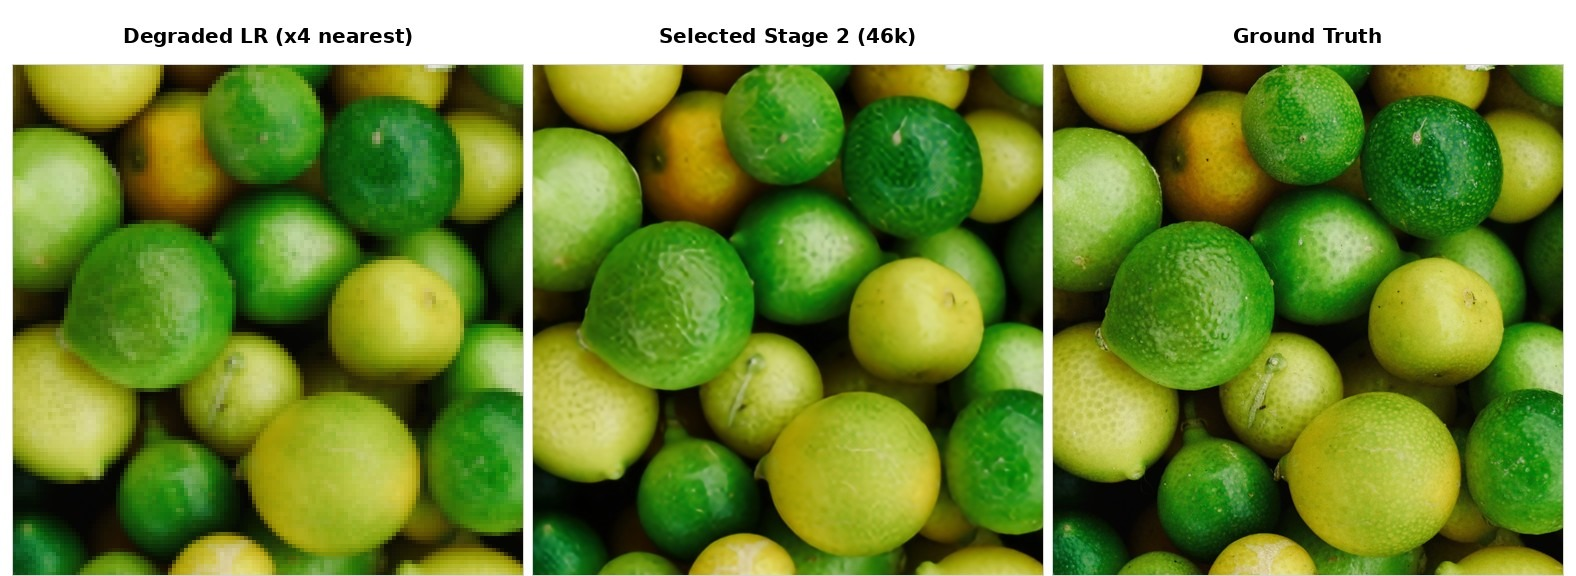
\includegraphics{../docs/assets/stage2_multiscale_demo.jpg}

\emph{Figure 1. Multiscale Stage 2 restores the degraded input while
retaining a visible fine-texture gap to ground truth.}

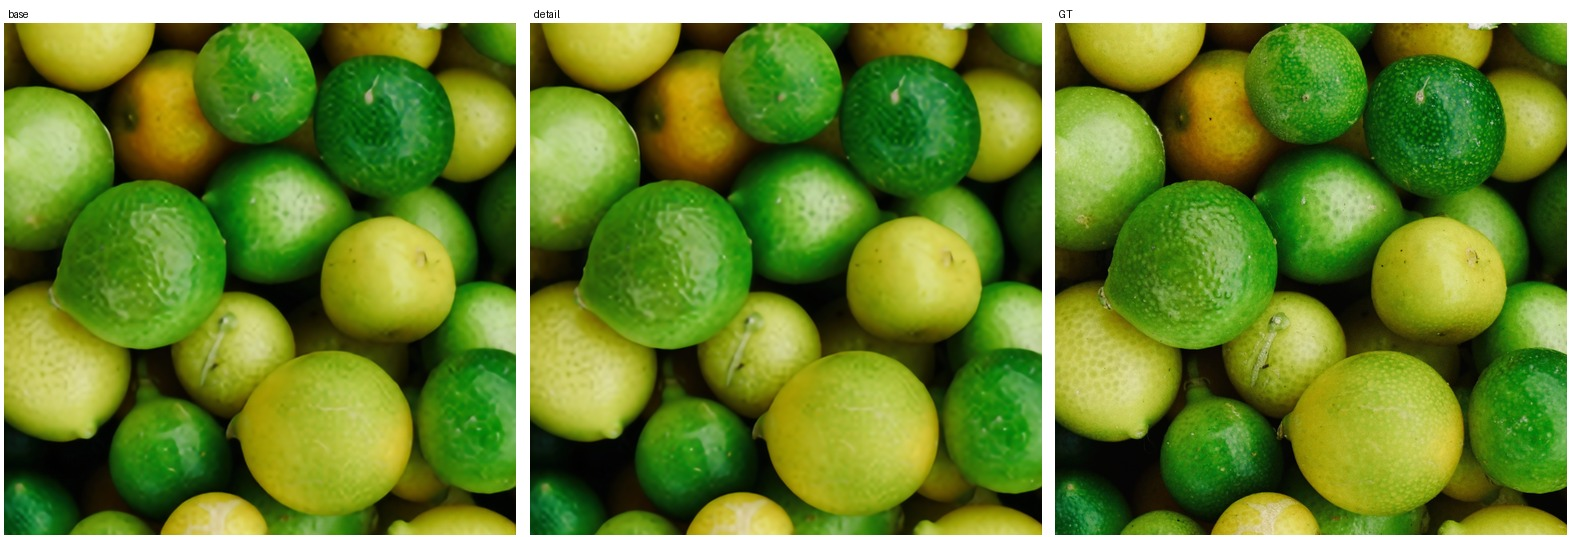
\includegraphics{../docs/assets/detail_branch_v1d_lime_demo.jpg}

\emph{Figure 2. Selected detail branch v1d adds a controlled,
artifact-light correction over the base; this illustrates both its
improvement and its remaining conservative behavior.}

\hypertarget{stage-2-multiscale-redesign}{%
\section{Stage 2 Multiscale
Redesign}\label{stage-2-multiscale-redesign}}

A decoded pixel/edge/highpass fine-tuning probe confirmed that the flat
Stage 2 condition predictor is the current bottleneck. By step 4000,
decoded PSNR had risen from \texttt{23.7387} to \texttt{24.2792}, but
the Laplacian detail ratio fell from \texttt{0.2817} to \texttt{0.2773}
and fixed samples remained visibly smooth. This is consistent with the
distortion-perception limitation of optimizing reconstruction losses
without sufficient spatial context or high-quality training exposure.

The replacement keeps all parameters and names of the selected
19M-parameter step 72000 predictor, then adds a zero-output-initialized
128-to-64-to-32 multiscale context branch. Partial initialization
therefore exactly preserves the previous output before training. The
training manifest also changes from 100,000 COCO plus 3,450
DIV2K/Flickr2K rows to a roughly balanced exposure of 100,000 COCO and
103,500 repeated DIV2K/Flickr2K rows. Random crops and degradations
remain stochastic, so repeated high-quality rows generate different
training pairs.

The design is informed by broad-context and multiscale restoration
findings in \href{https://arxiv.org/abs/2108.10257}{SwinIR},
\href{https://arxiv.org/abs/2309.05239}{HAT}, and
\href{https://arxiv.org/abs/2204.04676}{NAFNet}, together with the
data/degradation emphasis of
\href{https://arxiv.org/abs/2107.10833}{Real-ESRGAN}. The resulting
55.50M-parameter model passed a full batch-8 forward/backward and val100
smoke test on one L40S at approximately \texttt{34.8/46.1GB} VRAM and
\texttt{100\%} GPU utilization. The 50,000-micro-step long run is
tracked at \url{https://wandb.ai/jwheo/LuSIR/runs/6zt2do4v}.

The run completed normally. Step 46000 was selected over the final
checkpoint because it provides the best cross-preset distortion/detail
compromise. It improves the previous Stage 2 by \texttt{+1.0348\ dB} on
\texttt{photo\_detail\_mix} and \texttt{+0.9228\ dB} on \texttt{mild},
with \texttt{99/100} and \texttt{97/100} per-image wins and slightly
higher detail ratios. On the stronger \texttt{photo\_v2} and
\texttt{photo\_v3\_noise\_mix} presets it improves PSNR by
\texttt{+0.9441\ dB} and \texttt{+0.9650\ dB}, but the detail ratio
drops from roughly \texttt{0.29-0.30} to \texttt{0.22-0.23}. Visual
comparison confirms that the model improves color, large boundaries, and
denoising without convincingly recovering missing fur, text, fabric, or
distant texture. The experiment is a successful base-reconstruction
redesign but not a solution to perceptual fine-detail recovery.

An optional continuation completed from step 46000 using frozen ImageNet
VGG16 features at shallow and intermediate layers. This explicitly
introduces pretrained vision feature supervision, while still avoiding
pretrained text-to-image or generative models. A CUDA smoke test passed
at batch 4 with approximately \texttt{20.6/46.1GB} VRAM and
\texttt{2.62} micro-steps/s. The run completed 12,000 micro-steps. Step
8000 had the best shortlist score, \texttt{26.0092}, and improved
decoded PSNR over initialization by \texttt{+0.0101} to
\texttt{+0.0256\ dB} across the four tested presets. Step 11000 was
strongest on cleaner presets but regressed
\texttt{photo\_v3\_noise\_mix} by \texttt{-0.0063\ dB}. Fixed contact
sheets showed almost no visible difference from initialization, and
missing fine texture remained smoothed. The run is preserved as a
partial metric/latent success but is not promoted into the public path.
The completed run is tracked at
\url{https://wandb.ai/jwheo/LuSIR/runs/nrqhw05u}.

\hypertarget{dual-context-unique-data-stage-2-scale-up}{%
\section{Dual-Context Unique-Data Stage 2
Scale-up}\label{dual-context-unique-data-stage-2-scale-up}}

The VGG continuation\textquotesingle s \texttt{+0.0101} to
\texttt{+0.0256\ dB} cross-preset improvements were not visually
distinguishable and did not recover missing texture. Capacity and data
uniqueness are therefore changed together instead of extending the same
objective again. The previous HQ-balanced manifest had 203,600 rows but
only 103,550 unique images because DIV2K and Flickr2K were repeatedly
exposed.

The new manifest adds 30,000 unique LSDIR images for 133,450 unique
training images plus the unchanged 100-image validation set. The
predictor retains the selected 55.50M-parameter multiscale model and
adds a second zero-output- initialized multiscale context branch.
Partial initialization exactly preserves the selected step 46000 output
before training while increasing capacity to 119.24M parameters.

The one-L40S smoke test reproduced the initial \texttt{24.48\ dB}
decoded PSNR and \texttt{0.291} detail ratio. Batch 8 with gradient
accumulation 4 used approximately \texttt{37.8/46.1GB} VRAM, reached
\texttt{99\%} GPU utilization, and sustained approximately \texttt{0.75}
micro-step/s. The completed long run targeted 100,000 micro-steps, or
25,000 optimizer updates. Evaluation ran every 1,000 micro-steps, while
ordinary milestone checkpoints were limited to every 5,000 micro-steps
to stay within the disk budget. The run is tracked at
\url{https://wandb.ai/jwheo/LuSIR/runs/4akqckxu}.

The run completed all 100,000 micro-steps. Step 98,000 is the automatic
\texttt{eval/decoded\_psnr} best checkpoint on
\texttt{photo\_detail\_mix}; step 100,000 is slightly better on stronger
degradations. Re-evaluated with the same comparison tool against
selected step 46,000, the gains are \texttt{+0.1362\ dB} on
\texttt{photo\_detail\_mix}, \texttt{+0.1086\ dB} on \texttt{mild},
\texttt{+0.0540\ dB} on \texttt{photo\_v2}, and \texttt{-0.0356\ dB} on
\texttt{photo\_v3\_noise\_mix} for the best checkpoint. The final
checkpoint changes those to \texttt{+0.1256}, \texttt{+0.1025},
\texttt{+0.0668}, and \texttt{+0.0132\ dB}. This is a modest
reconstruction improvement, not a solved perceptual-detail problem.

\hypertarget{high-frequency-detail-branch-v1}{%
\section{High-Frequency Detail Branch
v1}\label{high-frequency-detail-branch-v1}}

The latest deterministic detail candidate is an image-space detail
branch, not another Stage 4 continuation. The path is:

\begin{Shaded}
\begin{Highlighting}[]
\NormalTok{LR {-}\textgreater{} frozen Stage 2 dual{-}context condition {-}\textgreater{} frozen Stage 1 decoder {-}\textgreater{} base SR}
\NormalTok{base SR + bicubic LR upsample {-}\textgreater{} gated high{-}frequency detail branch {-}\textgreater{} detail SR}
\end{Highlighting}
\end{Shaded}

The branch predicts a bounded RGB residual and a per-pixel gate. The
residual is projected through a local highpass operation before being
added to the base SR, which limits the model\textquotesingle s ability
to change global color or low-frequency structure. The output
convolution is zero-initialized, so step 0 exactly reproduces the frozen
Stage 2 + Stage 1 base output.

Implemented files:

\begin{Shaded}
\begin{Highlighting}[]
\NormalTok{configs/detail\_branch\_v1\_photo130k\_lsdir.yaml}
\NormalTok{configs/detail\_branch\_v1b\_aug\_photo130k\_lsdir.yaml}
\NormalTok{configs/detail\_branch\_v1c\_condition\_open\_photo130k\_lsdir.yaml}
\NormalTok{configs/detail\_branch\_v1d\_deep3m\_photo130k\_lsdir\_3ep.yaml}
\NormalTok{configs/hf/detail\_branch\_v1d\_deep3m\_photo130k\_lsdir\_3ep.yaml}
\NormalTok{tools/train/train\_detail\_branch.py}
\NormalTok{tools/eval/run\_fixed\_review\_detail\_branch.py}
\NormalTok{tests/test\_detail\_branch.py}
\end{Highlighting}
\end{Shaded}

A four-micro-step smoke test completed
load/eval/backprop/update/checkpoint successfully. Step 0 matched the
base output exactly at \texttt{24.6188\ dB} val100 PSNR; after one
optimizer update, the branch produced a tiny \texttt{+0.00005\ dB}
aggregate PSNR delta and \texttt{69/100} wins versus base. This is only
an integration check, not a quality claim.

The first v1 run was stopped at 7800 micro-steps, or 0.234 epoch over
the 133450-image train manifest, because early samples showed that the
residual was safe but visually too small. The v1b run kept the same
model and loss, but added horizontal flips, texture-biased crop retry,
and weak HR color jitter while excluding rotation, vertical flip,
affine/perspective transforms, erasing, and mixup.

The v1b run completed 40000 micro-steps, equal to 10000 optimizer
updates with \texttt{grad\_accum\_steps:\ 4}. It selected step 39500 by
\texttt{eval/detail\_score}:

\begin{Shaded}
\begin{Highlighting}[]
\NormalTok{base PSNR:        24.6188}
\NormalTok{detail PSNR:      24.6649}
\NormalTok{PSNR delta:       +0.0461 dB}
\NormalTok{base SSIM:        0.80013}
\NormalTok{detail SSIM:      0.80281}
\NormalTok{SSIM delta:       +0.00268}
\NormalTok{mean PSNR delta:  +0.0575}
\NormalTok{wins vs base:     98/100}
\NormalTok{detail wins:      100/100}
\end{Highlighting}
\end{Shaded}

Different metrics peak at nearby checkpoints: PSNR delta is highest at
step 38500 (\texttt{+0.0489\ dB}), SSIM delta is highest at step 37000
(\texttt{+0.00336}), and the final step 40000 reaches
\texttt{+0.0444\ dB} PSNR and \texttt{+0.00277} SSIM with
\texttt{98/100} wins. The selected step 39500 remains preserved as the
earlier public detail artifact because it has the best combined detail
score from the completed v1b run. Qualitatively, it is artifact-light
and slightly sharper on texture-heavy crops, but still conservative and
below GT on fine surface detail. It remains a historical comparison
artifact; the later selected v1d checkpoint is exposed through the Colab
WebUI detail runner.

V1c initialized from the selected v1b checkpoint, exposed the frozen
Stage 2 condition latent directly to the image-space branch, increased
the bounded residual scale, and opened the gate slightly. The selected
step 6000 improves the fixed \texttt{photo\_detail\_mix} val100 base by
\texttt{+0.0554\ dB} aggregate PSNR and \texttt{+0.00332} SSIM with
\texttt{99/100} wins. This was better than v1b but plateaued quickly
enough to motivate a controlled capacity test.

V1d keeps the v1c width and objective but increases residual depth from
8 to 18 blocks, raising branch capacity from \texttt{1.35M} to
\texttt{3.02M} parameters. The original blocks are copied from v1c step
6000 and the ten appended blocks are identity-initialized, so the step-0
output exactly reproduces v1c. The run completed 100,086 micro-steps,
exactly three passes over the 133,450-image manifest at batch size 4,
and selected step 99,500 by \texttt{eval/detail\_score}.

On ordinary fixed \texttt{photo\_detail\_mix} val100, selected step
99,500 improves the frozen base by \texttt{+0.1646\ dB} aggregate PSNR,
\texttt{+0.1888\ dB} mean PSNR, and \texttt{+0.00647} SSIM with
\texttt{99/100} PSNR wins and \texttt{100/100} detail wins. On the
strict-bicubic five-crop diagnostic it reaches \texttt{31.9513\ dB},
improving the frozen base by \texttt{+0.2102\ dB}, v1c by
\texttt{+0.1358\ dB}, and winning \texttt{5/5} images. This is also
\texttt{+0.1266\ dB} above the early v1d step-9500 snapshot.

Final step 100,086 reaches a nearly identical strict-bicubic
\texttt{31.9516\ dB}, but selected step 99,500 is stronger on
ordinary-val aggregate PSNR, SSIM, highpass improvement, and the
combined detail score. Visual inspection shows no white-dot, grid, or
excessive-sharpening artifacts. The larger branch and long run therefore
produced meaningful stable progress, but still did not close the visible
fine-texture gap to ground truth. Further same-objective continuation or
simple capacity scaling is not planned.

\hypertarget{learned-detail-need-mask-and-masked-detail-branch-v2}{%
\section{Learned Detail-Need Mask and Masked Detail Branch
v2}\label{learned-detail-need-mask-and-masked-detail-branch-v2}}

The next experiment separated \texttt{where\ detail\ is\ missing} from
\texttt{what\ detail\ should\ be\ generated}. A compact
460,545-parameter predictor observes the frozen base reconstruction,
bicubic input, Stage-2 condition latent, and four inference-time detail
proxies. On fixed \texttt{photo\_detail\_mix} val100, predictor step
3250 raises pixel correlation with the GT-supervised detail-need target
from \texttt{0.5403} to \texttt{0.7456}, raises top-20\% missing-detail
capture from \texttt{0.3252} to \texttt{0.3861}, and lowers
excess-detail capture from \texttt{0.4838} to \texttt{0.4304}.

Masked detail branch v2 initializes from v1d step 99500 and applies the
frozen predictor as a soft spatial gate with a \texttt{0.05} floor. Two
independent continuations converged to nearly identical candidates:

\begin{longtable}[]{@{}lrrrr@{}}
\toprule\noalign{}
Checkpoint & Detail score & PSNR delta & Mean PSNR delta & SSIM delta \\
\midrule\noalign{}
\endhead
\bottomrule\noalign{}
\endlastfoot
step 36000 & 26.69528 & +0.18744 dB & +0.20521 dB & +0.00721 \\
selected step 38000 & \textbf{26.69601} & +0.18177 dB & +0.20432 dB &
\textbf{+0.00755} \\
\end{longtable}

Step 38000 is selected by the configured \texttt{eval/detail\_score}. No
new best appeared through step 50000, and fixed grids at steps 34000,
38000, and 48000 were nearly indistinguishable, so the run stopped
before its 20-epoch upper bound.

The predictor establishes that missing-detail localization is learnable
from inference-time observations. However, gating the same deterministic
L1/highpass-oriented branch does not visibly synthesize the missing fine
texture. Location selection and texture generation remain separate
problems. The next detail experiment should retain the frozen fidelity
base and learned mask, but train a small bounded head with mask-weighted
patch perceptual or adversarial supervision and explicit
lowpass/fidelity guardrails.

That direction is now implemented as the untrained masked detail v3
patch probe. It preserves the selected v2 generator and its bounded
highpass-only residual path, adds a frozen-VGG feature loss spatially
weighted by the learned mask, and adds a small conditional PatchGAN that
receives the frozen base reconstruction and real/fake high-frequency
content. The adversarial objective starts after a 500-micro-step warmup
with a deliberately small generator weight. No long-run result is
claimed yet.

The evaluator now reports lowpass drift and residual energy inside and
outside the learned mask. At the selected v2 initialization, the L40S
smoke baseline is \texttt{0.000198} lowpass drift and \texttt{0.004333}
outside-mask residual L1. These values, PSNR/SSIM, and fixed visual
grids are explicit stop criteria for the v3 probe; the experiment is
rejected if it creates repeated texture, ringing, white points, or
persistent fidelity regression.

During reproducibility review, the original single-image and
formal-benchmark inference paths were found to omit the learned
predictor even though training and validation applied it. The inference
and benchmark runners now load the predictor checkpoint and floor from
the HF config. V1d configs without a mask retain their previous
behavior.

The masked v2 checkpoint also completed the formal 219-image
clean-bicubic benchmark. Relative to v1d, Y PSNR improves by
\texttt{+0.0034}, \texttt{+0.0602}, \texttt{+0.0135}, and
\texttt{+0.0167\ dB} on DIV2K, Set5, Set14, and Urban100. The overall
gain is \texttt{+0.0114\ dB} Y PSNR and \texttt{+0.00118} Y SSIM. This
consistent but small gain supports the same conclusion as the fixed
grids: learned gating improves correction placement, but does not solve
visible texture synthesis.

\hypertarget{public-artifacts}{%
\section{Public Artifacts}\label{public-artifacts}}

The latest LuSIR public artifacts are stored in \texttt{jwheo/LuSIR} on
Hugging Face:

\begin{Shaded}
\begin{Highlighting}[]
\NormalTok{checkpoints/stage4\_photo100k\_xl\_edge\_b16\_best\_eval\_condition\_decoded.pt}
\NormalTok{checkpoints/residual\_refiner\_stage2\_xl\_mild\_best\_eval\_refined.pt}
\NormalTok{checkpoints/stage4\_photo100k\_xl\_teacher\_residual\_photo\_v3\_step\_0002000.pt}
\NormalTok{checkpoints/stage4\_photo100k\_xl\_teacher\_residual\_photo\_detail\_best8000.pt}
\NormalTok{checkpoints/residual\_refiner\_stage2\_xl\_photo\_detail\_v2\_best39000.pt}
\NormalTok{checkpoints/stage2\_photo100k\_multiscale\_hqmix\_step\_0046000.pt}
\NormalTok{checkpoints/stage2\_photo100k\_multiscale\_hqmix\_perceptual\_step\_0008000.pt}
\NormalTok{checkpoints/stage2\_photo130k\_lsdir\_dual\_multiscale\_best98000.pt}
\NormalTok{checkpoints/detail\_branch\_v1b\_aug\_photo130k\_lsdir\_best39500.pt}
\NormalTok{checkpoints/detail\_branch\_v1d\_deep3m\_photo130k\_lsdir\_best99500.pt}
\NormalTok{checkpoints/detail\_mask\_predictor\_v1\_best3250.pt}
\NormalTok{checkpoints/detail\_branch\_v2\_masked\_photo130k\_lsdir\_best38000.pt}
\NormalTok{metrics/stage4\_photo100k\_xl\_edge\_b16\_val100\_t50\_32step\_summary.json}
\NormalTok{metrics/diagnose\_stage2\_xl\_residuals\_mild\_val100\_summary.json}
\NormalTok{metrics/residual\_refiner\_stage2\_xl\_mild\_probe\_early\_stop\_summary.json}
\NormalTok{metrics/eval\_residual\_refiner\_stage2\_xl\_photo\_v3\_noise\_mix\_val100\_summary.json}
\NormalTok{metrics/stage4\_photo100k\_xl\_teacher\_residual\_photo\_v3\_step2000\_val100\_t25\_32step\_summary.json}
\NormalTok{metrics/stage4\_photo100k\_xl\_teacher\_residual\_photo\_v3\_step2000\_val100\_t50\_32step\_summary.json}
\NormalTok{metrics/stage4\_photo100k\_xl\_teacher\_residual\_photo\_detail\_best8000\_val100\_t25\_summary.json}
\NormalTok{metrics/residual\_refiner\_stage2\_xl\_photo\_detail\_v2\_long\_summary.json}
\NormalTok{metrics/residual\_refiner\_v2\_best39000\_strength\_sweep\_summary.json}
\NormalTok{metrics/eval\_residual\_refiner\_v2\_best39000\_stage2\_xl\_mild\_val100\_summary.json}
\NormalTok{metrics/eval\_residual\_refiner\_v2\_best39000\_stage2\_xl\_photo\_v2\_val100\_summary.json}
\NormalTok{metrics/eval\_residual\_refiner\_v2\_best39000\_stage2\_xl\_photo\_v3\_noise\_mix\_val100\_summary.json}
\NormalTok{metrics/stage2\_multiscale\_hqmix\_step46000\_cross\_preset\_summary.json}
\NormalTok{metrics/stage2\_multiscale\_perceptual\_photo\_detail\_mix\_candidates.json}
\NormalTok{metrics/stage2\_multiscale\_perceptual\_mild\_candidates.json}
\NormalTok{metrics/stage2\_multiscale\_perceptual\_photo\_v2\_candidates.json}
\NormalTok{metrics/stage2\_multiscale\_perceptual\_photo\_v3\_noise\_mix\_candidates.json}
\NormalTok{metrics/stage2\_photo130k\_lsdir\_dual\_multiscale\_final\_summary.json}
\NormalTok{metrics/detail\_branch\_v1b\_aug\_photo130k\_lsdir\_summary.json}
\NormalTok{metrics/detail\_branch\_v1d\_deep3m\_photo130k\_lsdir\_3ep\_summary.json}
\NormalTok{metrics/benchmark\_bicubic5\_detail\_v1d\_best99500\_summary.json}
\NormalTok{metrics/detail\_branch\_v2\_masked\_photo130k\_lsdir\_summary.json}
\NormalTok{metrics/formal\_x4\_benchmark\_detail\_v2\_masked\_summary.json}
\NormalTok{metrics/formal\_x4\_benchmark\_detail\_v2\_masked\_metrics.csv}
\NormalTok{metrics/formal\_x4\_benchmark\_stage2\_detail\_perceptual\_v1\_summary.json}
\NormalTok{metrics/formal\_x4\_benchmark\_stage2\_detail\_perceptual\_v1\_metrics.csv}
\NormalTok{metrics/formal\_x4\_benchmark\_stage2\_detail\_perceptual\_v1\_delta\_crop\_selection.csv}
\NormalTok{samples/stage4\_photo100k\_xl\_edge\_b16\_val100\_t50\_32step\_grid\_lr\_bicubic\_sr\_gt.png}
\NormalTok{samples/diagnose\_stage2\_xl\_residuals\_mild\_val100\_grid.png}
\NormalTok{samples/residual\_refiner\_stage2\_xl\_mild\_probe\_step500\_grid.png}
\NormalTok{samples/eval\_residual\_refiner\_stage2\_xl\_photo\_v3\_noise\_mix\_val100\_grid.png}
\NormalTok{samples/compare\_residual\_refiner\_vs\_stage4\_edge\_0801\_photo\_v3.png}
\NormalTok{samples/stage4\_photo100k\_xl\_teacher\_residual\_photo\_v3\_step2000\_val100\_t25\_grid.png}
\NormalTok{samples/stage4\_photo100k\_xl\_teacher\_residual\_photo\_detail\_best8000\_val100\_t25\_grid.png}
\NormalTok{samples/residual\_refiner\_stage2\_xl\_photo\_detail\_v2\_best39000\_grid.png}
\NormalTok{samples/eval\_residual\_refiner\_v2\_best39000\_stage2\_xl\_mild\_val100\_grid.png}
\NormalTok{samples/eval\_residual\_refiner\_v2\_best39000\_stage2\_xl\_photo\_v2\_val100\_grid.png}
\NormalTok{samples/eval\_residual\_refiner\_v2\_best39000\_stage2\_xl\_photo\_v3\_noise\_mix\_val100\_grid.png}
\NormalTok{samples/stage2\_multiscale\_hqmix\_checkpoint\_comparison.png}
\NormalTok{samples/stage2\_multiscale\_perceptual\_photo\_detail\_mix\_candidates.png}
\NormalTok{samples/stage2\_multiscale\_perceptual\_photo\_v3\_noise\_mix\_candidates.png}
\NormalTok{samples/stage2\_dual\_lsdir\_photo\_detail\_mix\_best98k\_final100k\_contact\_sheet.png}
\NormalTok{samples/stage2\_dual\_lsdir\_mild\_best98k\_final100k\_contact\_sheet.png}
\NormalTok{samples/stage2\_dual\_lsdir\_photo\_v2\_best98k\_final100k\_contact\_sheet.png}
\NormalTok{samples/stage2\_dual\_lsdir\_photo\_v3\_noise\_mix\_best98k\_final100k\_contact\_sheet.png}
\NormalTok{samples/detail\_branch\_v1b\_aug\_photo130k\_lsdir\_best39500\_grid.png}
\NormalTok{samples/detail\_branch\_v1d\_deep3m\_photo130k\_lsdir\_best99500\_grid.png}
\NormalTok{samples/benchmark\_bicubic5\_detail\_v1d\_best99500\_grid.png}
\NormalTok{samples/detail\_branch\_v2\_masked\_photo130k\_lsdir\_best38000\_grid.png}
\NormalTok{samples/stage2\_detail\_perceptual\_v1\_benchmark\_delta\_crop\_sheet.jpg}
\NormalTok{configs/diffusion\_photo100k\_xl\_stage4\_condition\_v3\_edge\_b16.yaml}
\NormalTok{configs/residual\_refiner\_stage2\_xl\_mild\_probe.yaml}
\NormalTok{configs/diffusion\_photo100k\_xl\_stage4\_condition\_v3\_teacher\_residual\_photo\_v3\_b8\_probe.yaml}
\NormalTok{configs/diffusion\_photo100k\_xl\_stage4\_condition\_v3\_teacher\_residual\_photo\_detail\_b8\_long.yaml}
\NormalTok{configs/residual\_refiner\_stage2\_xl\_photo\_detail\_v2\_continue\_40k.yaml}
\NormalTok{configs/hf/residual\_refiner\_stage2\_xl\_photo\_detail\_v2.yaml}
\NormalTok{configs/latent\_pretrain\_photo100k\_multiscale\_hqmix\_perceptual\_continue.yaml}
\NormalTok{configs/latent\_pretrain\_photo130k\_lsdir\_dual\_multiscale\_long.yaml}
\NormalTok{configs/detail\_branch\_v1\_photo130k\_lsdir.yaml}
\NormalTok{configs/detail\_branch\_v1b\_aug\_photo130k\_lsdir.yaml}
\NormalTok{configs/hf/detail\_branch\_v1b\_aug\_photo130k\_lsdir.yaml}
\NormalTok{configs/detail\_branch\_v1d\_deep3m\_photo130k\_lsdir\_3ep.yaml}
\NormalTok{configs/hf/detail\_branch\_v1d\_deep3m\_photo130k\_lsdir\_3ep.yaml}
\NormalTok{configs/hf/detail\_mask\_predictor\_v1.yaml}
\NormalTok{configs/hf/detail\_branch\_v2\_masked\_photo130k\_lsdir.yaml}
\end{Highlighting}
\end{Shaded}

\hypertarget{next-work}{%
\section{Next Work}\label{next-work}}

The selected residual refiner remains the public Colab default, while
detail branch v1d and masked detail branch v2 are selectable
single-image/tiled Colab research options. The completed perceptual
Stage 2 continuation is not promoted. Candidate next steps are:

\begin{itemize}
\tightlist
\item
  preserve the deterministic base and validated learned detail-need
  mask, then test a small bounded mask-weighted patch
  perceptual/adversarial head;
\item
  select the generative path with LPIPS, DISTS, fixed visual review,
  high-frequency metrics, lowpass drift, and seed diversity instead of
  PSNR alone;
\item
  continue Stage 2/base architecture research as a separate
  clean-fidelity track for the measured \texttt{0.9235\ dB} DIV2K gap,
  rather than mixing that goal into the generative detail objective;
\item
  because v1d remains visually conservative and noise-MSE residual
  diffusion collapses toward zero, prioritize patch-level perceptual or
  adversarial supervision instead of increasing branch capacity again;
\item
  keep a degradation-aware gate or strong-input guardrail as the primary
  response to the remaining strong-preset failure tail.
\end{itemize}

The first latent residual probe increased high-frequency energy but
worsened GT-aligned detail and was stopped. The replacement diffuses
only signed Haar high bands of the image-space residual over the frozen
v1d base. Its clipped oracle improves the val8 base from
\texttt{28.7012} to \texttt{31.4039} dB, confirming that the
representation can express useful corrections. The step-20,000
condition-start continuation removed the early stochastic grain, but the
residual magnitude and seed diversity also collapsed toward zero. On
val100, start timesteps 15, 25, and 50 trail the v1d base by
\texttt{0.0880}, \texttt{0.1392}, and \texttt{0.3152} dB respectively,
and all settings worsen GT-aligned Laplacian and highpass error. The
result is not promoted, and the same noise-MSE objective will not be
continued. The next generative detail experiment should use an explicit
learned detail-need mask plus patch-level perceptual or adversarial
supervision rather than relying on conditional-mean residual prediction.
Implementation and evaluation details are in
\texttt{docs/HIGH\_FREQUENCY\_RESIDUAL\_DIFFUSION\_KO.md}.

The learned-mask prerequisite was subsequently trained as a compact
460,545-parameter predictor using the frozen fidelity base, bicubic
image, Stage-2 condition latent, and four observable detail proxies. On
the fixed photo-detail val100 set, it improved pixel correlation with
the supervised detail-need target from \texttt{0.5403} to
\texttt{0.7456}, improved top-20\% missing-detail capture from
\texttt{0.3252} to \texttt{0.3861}, and reduced excess-detail capture
from \texttt{0.4838} to \texttt{0.4304}. This clears the predefined
localization gate, but does not by itself establish improved SR output.
The subsequent masked v2 branch modestly improved ordinary val100
metrics but remained visually close to v1d and plateaued by step 38000.
Therefore the same deterministic objective will not be continued; the
next experiment must change texture-generation supervision while keeping
the validated spatial gate and fidelity guardrails.

\end{document}
